%\documentclass{standalone}
%\usepackage{tikz}
%\usetikzlibrary{patterns,plotmarks}
%\begin{document}
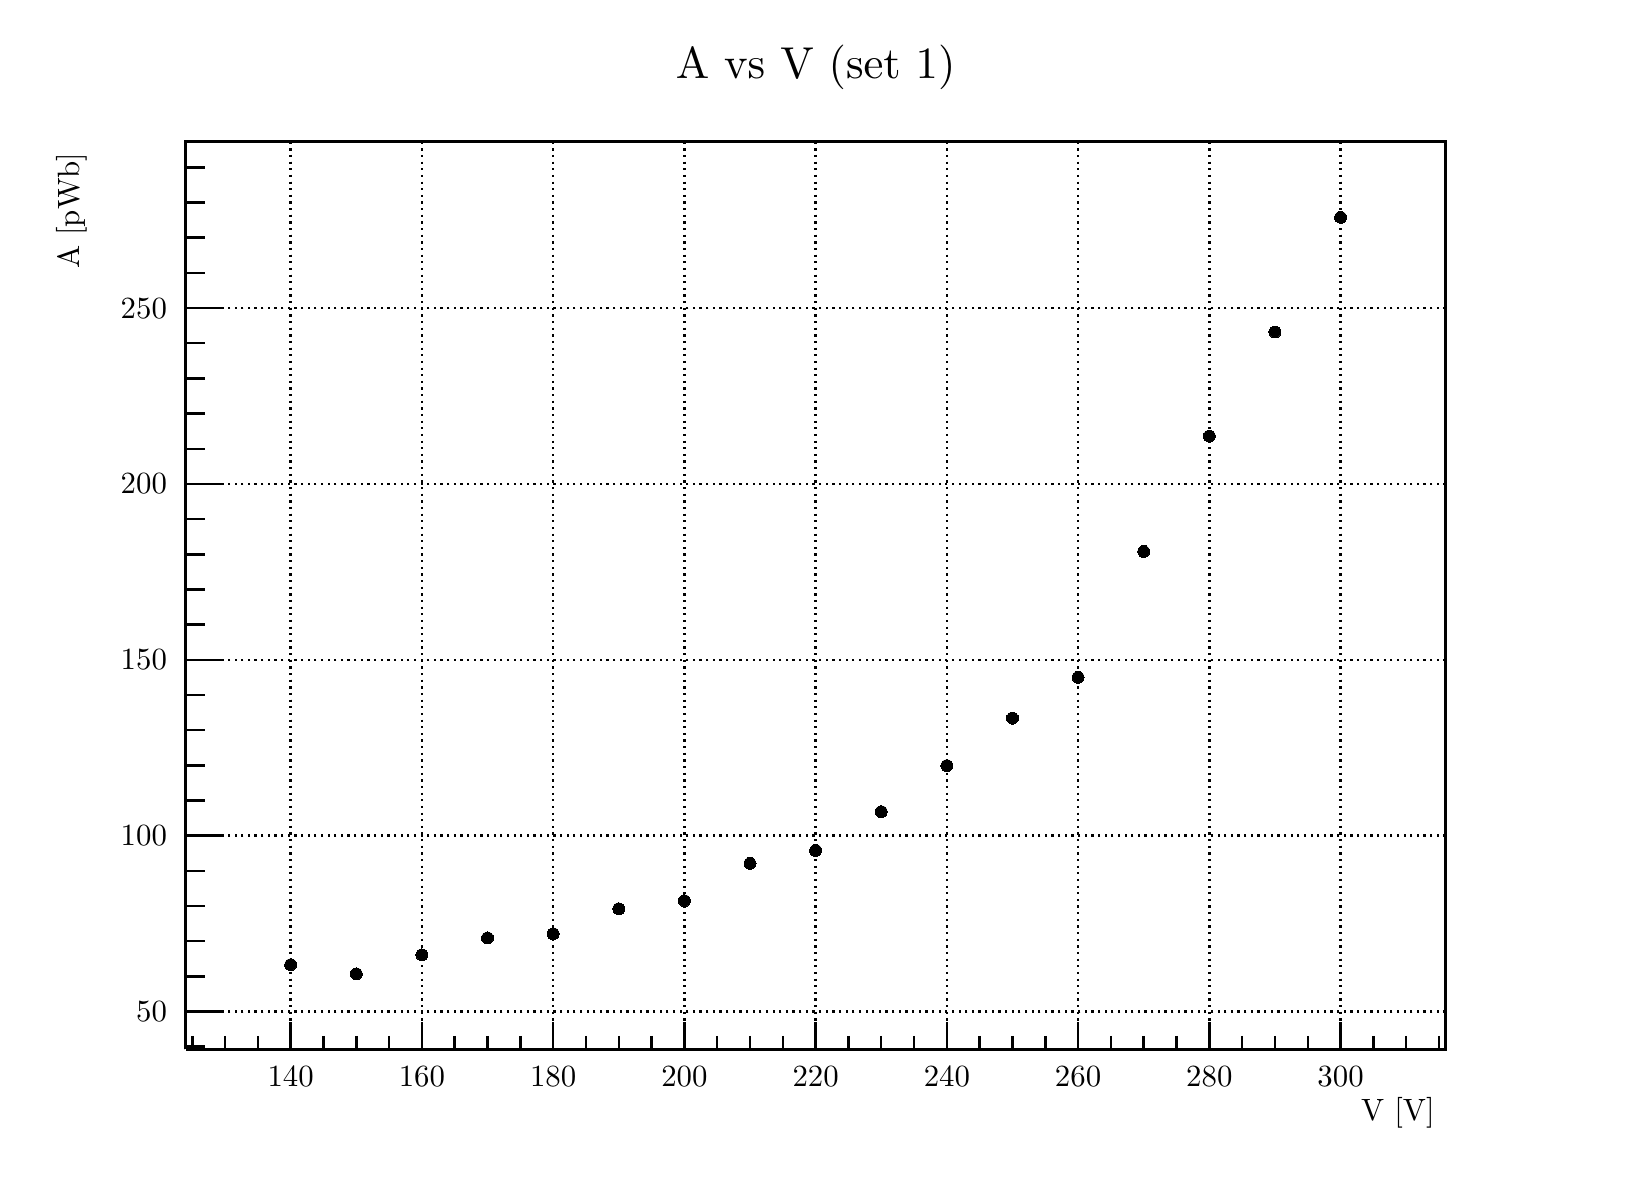
\begin{tikzpicture}
\def\CheckTikzLibraryLoaded#1{ \ifcsname tikz@library@#1@loaded\endcsname \else \PackageWarning{tikz}{usetikzlibrary{#1} is missing in the preamble.} \fi }
\CheckTikzLibraryLoaded{patterns}
\CheckTikzLibraryLoaded{plotmarks}
\pgfdeclareplotmark{cross} {
\pgfpathmoveto{\pgfpoint{-0.3\pgfplotmarksize}{\pgfplotmarksize}}
\pgfpathlineto{\pgfpoint{+0.3\pgfplotmarksize}{\pgfplotmarksize}}
\pgfpathlineto{\pgfpoint{+0.3\pgfplotmarksize}{0.3\pgfplotmarksize}}
\pgfpathlineto{\pgfpoint{+1\pgfplotmarksize}{0.3\pgfplotmarksize}}
\pgfpathlineto{\pgfpoint{+1\pgfplotmarksize}{-0.3\pgfplotmarksize}}
\pgfpathlineto{\pgfpoint{+0.3\pgfplotmarksize}{-0.3\pgfplotmarksize}}
\pgfpathlineto{\pgfpoint{+0.3\pgfplotmarksize}{-1.\pgfplotmarksize}}
\pgfpathlineto{\pgfpoint{-0.3\pgfplotmarksize}{-1.\pgfplotmarksize}}
\pgfpathlineto{\pgfpoint{-0.3\pgfplotmarksize}{-0.3\pgfplotmarksize}}
\pgfpathlineto{\pgfpoint{-1.\pgfplotmarksize}{-0.3\pgfplotmarksize}}
\pgfpathlineto{\pgfpoint{-1.\pgfplotmarksize}{0.3\pgfplotmarksize}}
\pgfpathlineto{\pgfpoint{-0.3\pgfplotmarksize}{0.3\pgfplotmarksize}}
\pgfpathclose
\pgfusepathqstroke
}
\pgfdeclareplotmark{cross*} {
\pgfpathmoveto{\pgfpoint{-0.3\pgfplotmarksize}{\pgfplotmarksize}}
\pgfpathlineto{\pgfpoint{+0.3\pgfplotmarksize}{\pgfplotmarksize}}
\pgfpathlineto{\pgfpoint{+0.3\pgfplotmarksize}{0.3\pgfplotmarksize}}
\pgfpathlineto{\pgfpoint{+1\pgfplotmarksize}{0.3\pgfplotmarksize}}
\pgfpathlineto{\pgfpoint{+1\pgfplotmarksize}{-0.3\pgfplotmarksize}}
\pgfpathlineto{\pgfpoint{+0.3\pgfplotmarksize}{-0.3\pgfplotmarksize}}
\pgfpathlineto{\pgfpoint{+0.3\pgfplotmarksize}{-1.\pgfplotmarksize}}
\pgfpathlineto{\pgfpoint{-0.3\pgfplotmarksize}{-1.\pgfplotmarksize}}
\pgfpathlineto{\pgfpoint{-0.3\pgfplotmarksize}{-0.3\pgfplotmarksize}}
\pgfpathlineto{\pgfpoint{-1.\pgfplotmarksize}{-0.3\pgfplotmarksize}}
\pgfpathlineto{\pgfpoint{-1.\pgfplotmarksize}{0.3\pgfplotmarksize}}
\pgfpathlineto{\pgfpoint{-0.3\pgfplotmarksize}{0.3\pgfplotmarksize}}
\pgfpathclose
\pgfusepathqfillstroke
}
\pgfdeclareplotmark{newstar} {
\pgfpathmoveto{\pgfqpoint{0pt}{\pgfplotmarksize}}
\pgfpathlineto{\pgfqpointpolar{44}{0.5\pgfplotmarksize}}
\pgfpathlineto{\pgfqpointpolar{18}{\pgfplotmarksize}}
\pgfpathlineto{\pgfqpointpolar{-20}{0.5\pgfplotmarksize}}
\pgfpathlineto{\pgfqpointpolar{-54}{\pgfplotmarksize}}
\pgfpathlineto{\pgfqpointpolar{-90}{0.5\pgfplotmarksize}}
\pgfpathlineto{\pgfqpointpolar{234}{\pgfplotmarksize}}
\pgfpathlineto{\pgfqpointpolar{198}{0.5\pgfplotmarksize}}
\pgfpathlineto{\pgfqpointpolar{162}{\pgfplotmarksize}}
\pgfpathlineto{\pgfqpointpolar{134}{0.5\pgfplotmarksize}}
\pgfpathclose
\pgfusepathqstroke
}
\pgfdeclareplotmark{newstar*} {
\pgfpathmoveto{\pgfqpoint{0pt}{\pgfplotmarksize}}
\pgfpathlineto{\pgfqpointpolar{44}{0.5\pgfplotmarksize}}
\pgfpathlineto{\pgfqpointpolar{18}{\pgfplotmarksize}}
\pgfpathlineto{\pgfqpointpolar{-20}{0.5\pgfplotmarksize}}
\pgfpathlineto{\pgfqpointpolar{-54}{\pgfplotmarksize}}
\pgfpathlineto{\pgfqpointpolar{-90}{0.5\pgfplotmarksize}}
\pgfpathlineto{\pgfqpointpolar{234}{\pgfplotmarksize}}
\pgfpathlineto{\pgfqpointpolar{198}{0.5\pgfplotmarksize}}
\pgfpathlineto{\pgfqpointpolar{162}{\pgfplotmarksize}}
\pgfpathlineto{\pgfqpointpolar{134}{0.5\pgfplotmarksize}}
\pgfpathclose
\pgfusepathqfillstroke
}
\definecolor{c}{rgb}{1,1,1};
\draw [color=c, fill=c] (0,0) rectangle (20,14.411);
\draw [color=c, fill=c] (2,1.4411) rectangle (18,12.9699);
\definecolor{c}{rgb}{0,0,0};
\draw [c,line width=0.9] (2,1.4411) -- (2,12.9699) -- (18,12.9699) -- (18,1.4411) -- (2,1.4411);
\definecolor{c}{rgb}{1,1,1};
\draw [color=c, fill=c] (2,1.4411) rectangle (18,12.9699);
\definecolor{c}{rgb}{0,0,0};
\draw [c,line width=0.9] (2,1.4411) -- (2,12.9699) -- (18,12.9699) -- (18,1.4411) -- (2,1.4411);
\draw [c,line width=0.9] (2,1.4411) -- (18,1.4411);
\draw [c,dash pattern=on 0.80pt off 1.60pt ,line width=0.9] (3.33333,12.9699) -- (3.33333,1.4411);
\draw [c,dash pattern=on 0.80pt off 1.60pt ,line width=0.9] (5,12.9699) -- (5,1.4411);
\draw [c,dash pattern=on 0.80pt off 1.60pt ,line width=0.9] (6.66667,12.9699) -- (6.66667,1.4411);
\draw [c,dash pattern=on 0.80pt off 1.60pt ,line width=0.9] (8.33333,12.9699) -- (8.33333,1.4411);
\draw [c,dash pattern=on 0.80pt off 1.60pt ,line width=0.9] (10,12.9699) -- (10,1.4411);
\draw [c,dash pattern=on 0.80pt off 1.60pt ,line width=0.9] (11.6667,12.9699) -- (11.6667,1.4411);
\draw [c,dash pattern=on 0.80pt off 1.60pt ,line width=0.9] (13.3333,12.9699) -- (13.3333,1.4411);
\draw [c,dash pattern=on 0.80pt off 1.60pt ,line width=0.9] (15,12.9699) -- (15,1.4411);
\draw [c,dash pattern=on 0.80pt off 1.60pt ,line width=0.9] (16.6667,12.9699) -- (16.6667,1.4411);
\draw [c,dash pattern=on 0.80pt off 1.60pt ,line width=0.9] (3.33333,12.9699) -- (3.33333,1.4411);
\draw [c,dash pattern=on 0.80pt off 1.60pt ,line width=0.9] (16.6667,12.9699) -- (16.6667,1.4411);
\draw [c,line width=0.9] (2,1.4411) -- (2,12.9699);
\draw [c,dash pattern=on 0.80pt off 1.60pt ,line width=0.9] (18,1.92393) -- (2,1.92393);
\draw [c,dash pattern=on 0.80pt off 1.60pt ,line width=0.9] (18,4.15716) -- (2,4.15716);
\draw [c,dash pattern=on 0.80pt off 1.60pt ,line width=0.9] (18,6.39039) -- (2,6.39039);
\draw [c,dash pattern=on 0.80pt off 1.60pt ,line width=0.9] (18,8.62361) -- (2,8.62361);
\draw [c,dash pattern=on 0.80pt off 1.60pt ,line width=0.9] (18,10.8568) -- (2,10.8568);
\draw [c,dash pattern=on 0.80pt off 1.60pt ,line width=0.9] (18,1.92393) -- (2,1.92393);
\draw [c,dash pattern=on 0.80pt off 1.60pt ,line width=0.9] (18,10.8568) -- (2,10.8568);
\draw [c,line width=0.9] (2,1.4411) -- (18,1.4411);
\draw [c,line width=0.9] (3.33333,1.78697) -- (3.33333,1.4411);
\draw [c,line width=0.9] (3.75,1.61404) -- (3.75,1.4411);
\draw [c,line width=0.9] (4.16667,1.61404) -- (4.16667,1.4411);
\draw [c,line width=0.9] (4.58333,1.61404) -- (4.58333,1.4411);
\draw [c,line width=0.9] (5,1.78697) -- (5,1.4411);
\draw [c,line width=0.9] (5.41667,1.61404) -- (5.41667,1.4411);
\draw [c,line width=0.9] (5.83333,1.61404) -- (5.83333,1.4411);
\draw [c,line width=0.9] (6.25,1.61404) -- (6.25,1.4411);
\draw [c,line width=0.9] (6.66667,1.78697) -- (6.66667,1.4411);
\draw [c,line width=0.9] (7.08333,1.61404) -- (7.08333,1.4411);
\draw [c,line width=0.9] (7.5,1.61404) -- (7.5,1.4411);
\draw [c,line width=0.9] (7.91667,1.61404) -- (7.91667,1.4411);
\draw [c,line width=0.9] (8.33333,1.78697) -- (8.33333,1.4411);
\draw [c,line width=0.9] (8.75,1.61404) -- (8.75,1.4411);
\draw [c,line width=0.9] (9.16667,1.61404) -- (9.16667,1.4411);
\draw [c,line width=0.9] (9.58333,1.61404) -- (9.58333,1.4411);
\draw [c,line width=0.9] (10,1.78697) -- (10,1.4411);
\draw [c,line width=0.9] (10.4167,1.61404) -- (10.4167,1.4411);
\draw [c,line width=0.9] (10.8333,1.61404) -- (10.8333,1.4411);
\draw [c,line width=0.9] (11.25,1.61404) -- (11.25,1.4411);
\draw [c,line width=0.9] (11.6667,1.78697) -- (11.6667,1.4411);
\draw [c,line width=0.9] (12.0833,1.61404) -- (12.0833,1.4411);
\draw [c,line width=0.9] (12.5,1.61404) -- (12.5,1.4411);
\draw [c,line width=0.9] (12.9167,1.61404) -- (12.9167,1.4411);
\draw [c,line width=0.9] (13.3333,1.78697) -- (13.3333,1.4411);
\draw [c,line width=0.9] (13.75,1.61404) -- (13.75,1.4411);
\draw [c,line width=0.9] (14.1667,1.61404) -- (14.1667,1.4411);
\draw [c,line width=0.9] (14.5833,1.61404) -- (14.5833,1.4411);
\draw [c,line width=0.9] (15,1.78697) -- (15,1.4411);
\draw [c,line width=0.9] (15.4167,1.61404) -- (15.4167,1.4411);
\draw [c,line width=0.9] (15.8333,1.61404) -- (15.8333,1.4411);
\draw [c,line width=0.9] (16.25,1.61404) -- (16.25,1.4411);
\draw [c,line width=0.9] (16.6667,1.78697) -- (16.6667,1.4411);
\draw [c,line width=0.9] (3.33333,1.78697) -- (3.33333,1.4411);
\draw [c,line width=0.9] (2.91667,1.61404) -- (2.91667,1.4411);
\draw [c,line width=0.9] (2.5,1.61404) -- (2.5,1.4411);
\draw [c,line width=0.9] (2.08333,1.61404) -- (2.08333,1.4411);
\draw [c,line width=0.9] (16.6667,1.78697) -- (16.6667,1.4411);
\draw [c,line width=0.9] (17.0833,1.61404) -- (17.0833,1.4411);
\draw [c,line width=0.9] (17.5,1.61404) -- (17.5,1.4411);
\draw [c,line width=0.9] (17.9167,1.61404) -- (17.9167,1.4411);
\draw [anchor=base] (3.33333,0.965539) node[scale=1.11327, color=c, rotate=0]{140};
\draw [anchor=base] (5,0.965539) node[scale=1.11327, color=c, rotate=0]{160};
\draw [anchor=base] (6.66667,0.965539) node[scale=1.11327, color=c, rotate=0]{180};
\draw [anchor=base] (8.33333,0.965539) node[scale=1.11327, color=c, rotate=0]{200};
\draw [anchor=base] (10,0.965539) node[scale=1.11327, color=c, rotate=0]{220};
\draw [anchor=base] (11.6667,0.965539) node[scale=1.11327, color=c, rotate=0]{240};
\draw [anchor=base] (13.3333,0.965539) node[scale=1.11327, color=c, rotate=0]{260};
\draw [anchor=base] (15,0.965539) node[scale=1.11327, color=c, rotate=0]{280};
\draw [anchor=base] (16.6667,0.965539) node[scale=1.11327, color=c, rotate=0]{300};
\draw [anchor= east] (18,0.634085) node[scale=1.11327, color=c, rotate=0]{V [V]};
\draw [c,line width=0.9] (2,1.4411) -- (2,12.9699);
\draw [c,line width=0.9] (2.48,1.92393) -- (2,1.92393);
\draw [c,line width=0.9] (2.24,2.37057) -- (2,2.37057);
\draw [c,line width=0.9] (2.24,2.81722) -- (2,2.81722);
\draw [c,line width=0.9] (2.24,3.26386) -- (2,3.26386);
\draw [c,line width=0.9] (2.24,3.71051) -- (2,3.71051);
\draw [c,line width=0.9] (2.48,4.15716) -- (2,4.15716);
\draw [c,line width=0.9] (2.24,4.6038) -- (2,4.6038);
\draw [c,line width=0.9] (2.24,5.05045) -- (2,5.05045);
\draw [c,line width=0.9] (2.24,5.49709) -- (2,5.49709);
\draw [c,line width=0.9] (2.24,5.94374) -- (2,5.94374);
\draw [c,line width=0.9] (2.48,6.39039) -- (2,6.39039);
\draw [c,line width=0.9] (2.24,6.83703) -- (2,6.83703);
\draw [c,line width=0.9] (2.24,7.28368) -- (2,7.28368);
\draw [c,line width=0.9] (2.24,7.73032) -- (2,7.73032);
\draw [c,line width=0.9] (2.24,8.17697) -- (2,8.17697);
\draw [c,line width=0.9] (2.48,8.62361) -- (2,8.62361);
\draw [c,line width=0.9] (2.24,9.07026) -- (2,9.07026);
\draw [c,line width=0.9] (2.24,9.51691) -- (2,9.51691);
\draw [c,line width=0.9] (2.24,9.96355) -- (2,9.96355);
\draw [c,line width=0.9] (2.24,10.4102) -- (2,10.4102);
\draw [c,line width=0.9] (2.48,10.8568) -- (2,10.8568);
\draw [c,line width=0.9] (2.48,1.92393) -- (2,1.92393);
\draw [c,line width=0.9] (2.24,1.47728) -- (2,1.47728);
\draw [c,line width=0.9] (2.48,10.8568) -- (2,10.8568);
\draw [c,line width=0.9] (2.24,11.3035) -- (2,11.3035);
\draw [c,line width=0.9] (2.24,11.7501) -- (2,11.7501);
\draw [c,line width=0.9] (2.24,12.1968) -- (2,12.1968);
\draw [c,line width=0.9] (2.24,12.6434) -- (2,12.6434);
\draw [anchor= east] (1.9,1.92393) node[scale=1.11327, color=c, rotate=0]{50};
\draw [anchor= east] (1.9,4.15716) node[scale=1.11327, color=c, rotate=0]{100};
\draw [anchor= east] (1.9,6.39039) node[scale=1.11327, color=c, rotate=0]{150};
\draw [anchor= east] (1.9,8.62361) node[scale=1.11327, color=c, rotate=0]{200};
\draw [anchor= east] (1.9,10.8568) node[scale=1.11327, color=c, rotate=0]{250};
\draw [anchor= east] (0.54812,12.9699) node[scale=1.11327, color=c, rotate=90]{A [pWb]};
\foreach \P in {(3.33333,2.51797), (4.16667,2.40184), (5,2.64303), (5.83333,2.85742), (6.66667,2.91101), (7.5,3.22813), (8.33333,3.33086), (9.16667,3.80431), (10,3.96956), (10.8333,4.46088), (11.6667,5.04598), (12.5,5.64895), (13.3333,6.16706),
 (14.1667,7.76605), (15,9.23105), (15.8333,10.5531), (16.6667,12.0092)}{\draw[mark options={color=c,fill=c},mark size=2.162162pt, line width=0.000000pt, mark=*] plot coordinates {\P};}
\draw (10,13.9179) node[scale=1.61424, color=c, rotate=0]{A vs V (set 1)};
\end{tikzpicture}
%\end{document}
